\chapter{Cronograma}\label{cap:cronograma}

Com o objetido de facilitar a pesquisa, optou-se por
fazer a seguinte divisão dos períodos de pesquisa:
\begin{description}
  \item Revisão Bibliográfica
  \item Enunciação do Problema
  \item Entendimento das Heurísticas
  \item Desenvolvimento dos Algorítimos
  \item Especificação dos algorítimos de avalição
\end{description}
Os prazos previstos para cada um dos respectivos periodos
podem ser visto na figura \ref{cron}.

\begin{figure}[h!]
  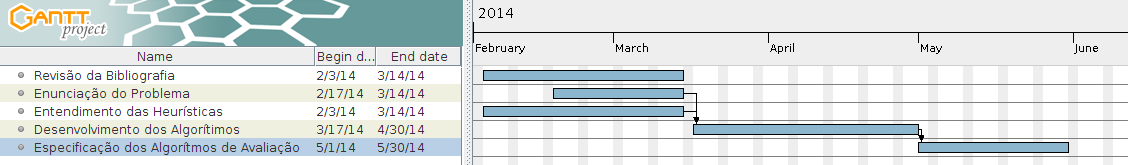
\includegraphics[width = \linewidth]{imgs/cronograma}
  \label{cron}
  \caption{Cronograma das atividades}
  
\end{figure}